\chapter{Basic Properties of Field}\label{chp:6_1}

\section{Rings and fields}

\begin{definition}{}{}
    A ring $(R,+,*)$ is a set $R$,
    together with two binary operations, denoted by $+$ and $*$,
    such that\\
    (1) $R$ is an abelian group with respect to $+$;\\
    (2) $R$ is closed under $*$.\\
    (3) $*$ is associative, that is $(a*b)*c=a*(b*c)$ for all $a,b,c\in R$;\\
    (4) the distributive laws hold, that is, for all $a,b,c\in R$ we have $a*(b+c)=(a*b)+(a*c)$
    and $(b+c)*a=(b*a)+(c*a)$.\\
    Typically, we use $0$ to denote the identity element of the abelian group $R$ with respect to addition,
    and $-a$ to denote the additive inverse of $a\in R$.
\end{definition}

\begin{definition}{}{}
    (1) A ring is called a ring with identity if the ring has a multiplicative identity (usually denoted $e$ or $1$).\\
    (2) A ring is called commutative if $*$ is commutative.\\
    (3) A ring is called an integral domain if it is a commutative ring with identity $e \neq 0$ in which
    $ab = 0$ implies $a = 0$ or $b = 0$ (i.e. no zero divisors).\\
    (3) A ring is called a division ring (or skew field) if the non-zero elements form a group under $*$.\\
    (4) A commutative division ring is called a field.
\end{definition}

So, in summary: a field is a set $F$ on which two binary operations, called addition and multiplication, 
are defined, and which contains two distinguished elements $e$ and $0$ with $0 \neq e$. 
Moreover, $F$ is an abelian group with respect to addition, having $0$ as the identity element, 
and the non-zero elements of $F$ (often written $F^*$) 
form an abelian group with respect to multiplication having $e$ as
the identity element. 
The two operations are linked by the distributive laws.


\begin{proposition}{}{}
    Every finite integral domain is a field.
\end{proposition}

\begin{definition}{}{}
    (1) A subset $S$ of a ring $R$ is called a subring of $R$ if
     $S$ is a subgroup of $R$ under $+$ (closed under addition and subtraction) and
        is closed under multiplication. \\
    (2) A subset $S$ of a ring $R$ is called an ideal if 
        $I$ is a subring of $R$ and for all $a \in I$ and $r \in R$
        we have $ar \in I$ and $ra \in I$.\\
    (3) Let $R$ be a commutative ring with an identity. 
        Then the smallest ideal containing an element
        $a \in R$ is $(a) := {ra : r \in R}$. We call $(a)$ the principal ideal generated by $a$.
\end{definition}

\begin{definition}{}{}
    An integral domain in which every ideal is principal is called a principal ideal domain (PID).
\end{definition}

An ideal $I$ of $R$ defines a partition of $R$ into disjoint cosets (with respect to $+$),
these form a ring with respect to the following operations:
\begin{align*}
    (a+I)+(b+I)=(a+b)+J,\\
    (a+I)(b+I)=ab+J.
\end{align*}
This ring is called the quotient ring and is denoted by $R/I$.

\begin{proposition}{}{}
    $\Z/(p)$, the ring of residue classes of the integers modulo the principal ideal generated by a prime $p$,
    is a field.
\end{proposition}
\begin{proof}
    proof of example\ref{exa:modulo prime is a field}.
\end{proof}

These are our first examples of finite fields!

\begin{theorem}{}{}
    Let $\sigma$ be a homomorphism from ring $R$ to ring $S$, then 
    the quotient ring $R/\text{ker}\sigma$ and the ring $Im\sigma$ 
    are isomorphic by the map $r+\text{ker}\sigma\mapsto \sigma(r)$.
\end{theorem}

We can use mappings to transfer a structure from an algebraic system to a set without structure.
Given a ring $R$, a set $S$ and a bijective map $\sigma:R\rightarrow S$,
we can use $\sigma$ to define a ring structure on $S$ that
converts $\sigma$ into an isomorphism. Sepcifically, for $s_1=\sigma(r_1)$ and $s_2=\sigma(r_2)$, define
\begin{align*}
    s_1+s_2 \text{ to be } \sigma(r_1+r_2) \text{ and } s_1s_2 \text{ to be } \sigma(r_1)\sigma(r_2).
\end{align*}
This is called the ring structure induced by $\sigma$; any extra properties of $R$ are inherited by $S$.
\par
This idea allows us to obtain a more convenient representation for the finite fields $\Z/(p)$.

\begin{definition}{}{}
    For a prime $p$, let $\F_p$ be the set $\{0,1,...,p-1\}$ of integers,
    and let $\sigma: \Z/(p)\rightarrow \F_p$ be the mapping defined by $\sigma(\bar{a})=a$ for $a=0,1,...,p-1$.
    Then $\F_p$ endowed with the field structure induced by $\sigma$ is a finite field, called the Galois field of order $p$.
\end{definition}

From above, the mapping $\sigma$ becomes an isomorphism, 
so $\sigma (\bar{a}+\bar{b})=\sigma (\bar{a}) + \sigma (\bar{b})$ and $\sigma(\bar{a}\bar{b})=\sigma(\bar{a})\sigma(\bar{b})$.
The finite field $\F_p$ has zero element $0$, identity element $1$ and its structure is that of $\Z/(p)$.
So, computing with element of $\F_p$ now means ordinary arithmetic of integers with reduction modulo $p$.

\begin{definition}{}{}
    If $R$ is an arbitrary ring and there exists a positive integer $n$ such that $nr=0$ for every $r\in R$
    (i.e. $r$ added to itself $n$ times is the zero element) then the least such positive integer $n$ is called
    the characteristic of $R$, and $R$ is said to have positive characteristic.
    If no such positive integer $n$ exists, $R$ is said to have characteristic $0$.
\end{definition}

\begin{proposition}{}{prime characteristic}
    A ring $R\neq \{0\}$ of positive characteristic with an identity and no zero divisors must have prime characteristic.
\end{proposition}
\begin{proof}
    Since $R$ contains non-zero elements, 
    it follows that $R$ has characteristic $n\geqs 2$.
    If $n$ were not prime, we could wirte $n=km$ with $k,m\in\Z$, $1<k,m<n$.
    Then $0=ne=(km)e=(ke)(me)$, so either $ke=0$ or $me=0$, since $R$ has no zero divisors.
    Hence either $kr=(ke)r=0$ for all $r\in R$ or $mr=(me)r=0$ for all $r\in R$, contradicting the definition of $n$ as the characteristic.
\end{proof}

\begin{corollary}{}{finite field prime characteristic}
    A finite field has prime characteristic.
\end{corollary}
\begin{proof}
    From proposition\ref{prop:prime characteristic}, 
    we need only show that a finite field $F$ has a positive characteristic.
    Consider the multiples $e,2e,3e,...$ of the identity. Since $F$ contains only finitely many elements,
    there must exist integers $k$ and $m$ with $1\leqs k<m$ such that $ke=me$, i.e. $(k-m)e=0$,
    and thus $(k-m)f=(k-m)ef=0f=0$ for all $f\in F$ so $F$ has a positive characteristic.
\end{proof}

\begin{example}{}{}
    The field $\Z/(p)$ (equivalently, $\F_p$) has characteristic $p$.
\end{example}

\begin{definition}{}{}
    A field containing no proper subfields is called a prime field.
\end{definition}

For example, $\F_p$ is a prime field, since any subfield must contain the elements $0$ and $1$, and since it
is closed under addition it must contain all other elements, i.e. it must be the whole field.

\begin{proposition}{}{}
    The intersection of all subfields of a field $F$ is a prime field, 
    called the prime subfield of $F$.
\end{proposition}

\begin{proposition}{}{prime subfield isomorphic to Q or Fp}
    The prime subfield of a field $F$ is isomorphic to $\Q$ 
    if $F$ has characteristic $0$ and 
    is isomorphic to $\F_p$
    if $F$ has characteristic $p$.
\end{proposition}

\section{Polynomials}

\begin{definition}{}{}
    Let $f=\sum\limits_{i=0}^{n}a_ix^i=a_0+a_1x+...+a_nx^n$
    be a Polynomial over $R$ which is not the zero polynomial, 
    so we can suppose $a_n\neq 0$. Then $n$ is called the degree of $f$.
    By convention, $deg(0)=-\infty$. Polynomials of degree $0$ are called constant polynomials.
    If the leading coefficient of $f$ is $1$ (the identity of $R$) then $f$ is called a monic polynomial.
\end{definition}

\begin{theorem}{}{}
    The set of polynomials over a ring $R$ forms a ring.
    It is called the polynomial ring over $R$ and denoted by $R[x]$.
    Its zero element is the zero polynomial, all of whose coefficients are zero. 
\end{theorem}

Let $F$ denote a (not necessarily finite) field. 
From now on, we consider polynomials over fields.
We say that the polynomial $g \in F[x]$ divides $f \in F[x]$
if there exists a polynomial $h \in F[x]$ such that $f = gh$.

\begin{theorem}{Division Algorithm}{}
    Let $g\neq 0$ be a polynomial in $F[x]$.
    Then for any $f\in F[x]$, there exists polynomial $q,r\in F[x]$
    such that
    \begin{align*}
        f=qg+r, \text{ where } \text{deg}(r)<\text{deg}(g).
    \end{align*}
\end{theorem}

Using the division algorithm, we can show that every ideal of $F[x]$ is principal.

\begin{proposition}{}{}
    $F[x]$ is a principal ideal domain. In fact,
    for every $I\neq (0)$ of $F[x]$ there is a uniquely determined monic polynomial 
    $g\in F[x]$ such that $I=(g)$.
\end{proposition}

\begin{proof}
    Let $I$ be an ideal in $F[x]$. If $I=\{0\}$, then $I=(0)$.
    If $I\neq \{0\}$, choose a non-zero polynomial $k\in I$ of smallest degree.
    Let $b$ be the leading coefficient of $k$, and set $m=b^{-1}k$.
    Then $m\in I$ and $m$ is monic. We will show: $I=(m)$.
    Clearly, $(m)\subset I$. Now take $f\in I$;
    by the division algorithm there are polynomial $q,r$ with $f=qm+r$ where 
    either $r=0$ or deg($r$)<deg($m$). Now, $r=f-qm\in I$.
    If $r\neq 0$, we contradict the minimality of $m$;
    so we must have $r=0$, i.e. $f$ is a multiple of $m$ and $I=(m)$.\\
    \par
    We now show uniqueness: if $m_1\in F[x]$ is another monic polynomial with $I=(m_1)$,
    then $m=c_1m_1$ and $m_1=c_2m$ with $c_1,c_2\in F[x]$. Then $m=c_1c_2m$, i.e. $c_1c_2=1$, 
    and so $c_1,c_2$ are constant polynomials.
    Since both $m$ and $m_1$ are monic, we must have $m=m_1$.
\end{proof}

We next introduce an important type of polynomial.

\begin{definition}{}{}
    A polynomial $p\in F[x]$ is said to be irreducible over $F$
    if $p$ has positive degree and $p=bc$ with $b,c\in F[x]$ implies that either $b$ or $c$ is a constant polynomial.
    A polynomial which does allow a non-trivial factorization over $F$ is called reducible over $F$.
\end{definition}
\begin{remark}
    Note that the field $F$ under consideration is all-important here,
    e.g. the polynomial $x^2+1$ is irreducible in $\R[x]$, 
    but reducible in $\C[x]$, where it factors as $(x+i)(x-i)$.
\end{remark}

\begin{theorem}{}{}
    Any polynomial $f\in F[x]$ of positive degreee an be written in the form
    \begin{align*}
        f=ap_1^{e_1}\cdots p_k^{e_k}
    \end{align*}
    where $a\in F$, $p_1,..., p_k$ are distinct monic irreducible
    in $F[x]$ and $e_1,...,e_k$ are positive integers.
    This factorization is unique and is called the canonical factorization of $f$ in $F[x]$.
\end{theorem}

\begin{example}{}{}
    Find all irreducible polynomials over $\F_2$ of degree $3$.
\end{example}

\begin{proof}
    The operation tables of $\F_2$ are:
    \begin{figure}[H]
        \centering
        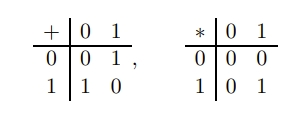
\includegraphics[width=0.3\textwidth]{figure/F_2_operator_table.png}
        \caption{}
    \end{figure}
    Since $\F_2=\{0,1\}$, it follows that a non-zero polynomial 
    in $\F_2[x]$ must be monic.
    The degree $3$ polynomials are of the form $x^3+ax^2+bx+c$,
    where each coefficient is $0$ or $1$, i.e. there are $2^3=8$ of them.\\
    If $c=0$, such a polynomial is reducible over $\F_2$ since it has $x$ as divisor.\\
    If $a=b=0,c=1$, assume $x^3+1=(x+a_0)(x^2+b_1x+b_0)=x^3+(b_1+a_0)x^2+(a_0b_1+b_0)x +a_0b_0$,
    then $a_0=b_0=b_1=1$ and so be reducible.\\
    If $a=b=c=1$, assume $x^3+x^2+x+1=(x+a_0)(x^2+b_1x+b_0)=x^3+(b_1+a_0)x^2+(a_0b_1+b_0)x +a_0b_0$,
    then $a_0=b_0=1$, $b_1=0$ and so be reducible.\\
    If $a=c=1$, $b=0$, assume $x^3+x^2+1=(x+a_0)(x^2+b_1x+b_0)=x^3+(b_1+a_0)x^2+(a_0b_1+b_0)x +a_0b_0$,
    then $a_0=b_0=1$, $b_1=0$ and so $a_0b_1+b_0=1\neq 0$. This is a contradiction and so be irreducible.\\
    If $b=c=1$, $a=0$, assume $x^3+x+1=(x+a_0)(x^2+b_1x+b_0)=x^3+(b_1+a_0)x^2+(a_0b_1+b_0)x +a_0b_0$,
    then $a_0=b_0=1$,$b_1=1$ and so $a_0b_1+b_0=0$. This is a contradiction and so be irreducible.\\
    Hence, $x^3+x^2+1$ and $x^3+x+1$ are irreducible.
\end{proof}

\begin{proposition}{}{}
    For $f \in F[x]$, 
    the quotient ring $F[x]/(f)$ is 
    a field if and only if 
    $f$ is irreducible over $F$.
\end{proposition}


% \begin{definition}{}{}
%     Let $F$ be a commutative ring with unity. 
%     $F$ is a field if $(F^*,\cdot)=(F\setminus\{0_F\},\cdot)$ is an abelian group.
% \end{definition}

% \begin{proposition}{}{}
%     Any finite subgroup of $F^*$ is cyclic.
% \end{proposition}

% \begin{proof}
%     proof referring to \href{https://proofwiki.org/wiki/Finite_Multiplicative_Subgroup_of_Field_is_Cyclic}{prook by proofwiki}
% \end{proof}


% \begin{proposition}{}{}
%     The only ideals of $F$ are $F$ and $(0)$.
% \end{proposition}

% \begin{proof}
%     proof referring to \ref{prop:field and ideals relation}
% \end{proof}

% \begin{proposition}{}{}
%     $F$ has no zero divisors.
% \end{proposition}
% \begin{proof}
    
% \end{proof}


\section{Reference}

\begin{itemize}
    \item \href{https://www.ma.imperial.ac.uk/~anskor/notesM2P4.pdf}{lecture note by anskor}
    \item \href{https://www.math.rwth-aachen.de/~Max.Neunhoeffer/Teaching/ff/ffchap1.pdf}{Introduction}
    \item \href{https://www.math.rwth-aachen.de/~Max.Neunhoeffer/Teaching/ff/ffchap2.pdf}{prime field}
\end{itemize}